\documentclass[12pt]{article}
\usepackage[pdftex]{graphicx}
\usepackage{listings}

\pagestyle{empty}
\setcounter{secnumdepth}{2}
\newcommand{\systemName}{Task Manager }
\topmargin=0cm
\oddsidemargin=0cm
\textheight=22.0cm
\textwidth=16cm
\parindent=0cm
\parskip=0.15cm
\topskip=0truecm
\raggedbottom
\abovedisplayskip=3mm
\belowdisplayskip=3mm
\abovedisplayshortskip=0mm
\belowdisplayshortskip=2mm
\normalbaselineskip=12pt
\normalbaselines

\begin{document}

\vspace*{0.5in}
\centerline{\bf\Large Requirements Document}

\vspace*{0.5in}
\centerline{\bf\Large Team 1}

\vspace*{0.5in}
\centerline{\bf\Large February 3, 2012}

\vspace*{1.5in}
\begin{table}[htbp]
\caption{Team}
\begin{center}
\begin{tabular}{|r | c|}
\hline
{\bf Name} & {\bf ID Number} \\
Jonathan Bergeron & 9764453 \\
Marc-Andr\'{e} Faucher & 9614729 \\
Jeffrey How & 9430954 \\
Dmitry Kuznetsov & 5679311 \\
William Ling & 9193480 \\
Thomas Paulin & 9333630 \\
Alain Sakha & 9770836 \\
Kai Wang & 5652723 \\
\hline
\end{tabular}
\end{center}
\end{table}

\clearpage

\section{System}

\subsection{Purpose}

The purpose of this document is to define requirements for the \systemName system. \\

The intended audience of this document is described in table 2. \\

% TABLE
\begin{table}[htbp]
\caption{Targeted audience of this document.}
\begin{center}
\begin{tabular}{|l | l|}
\hline
{\bf Group of the readers} & {\bf Reasons for reading}\\ \cline{1-2}
Users and customers & To give feedback about the requirements\\ \cline{1-2}
System developers & To understand what functions and properties the system \\&must contain\\ \cline{1-2}
Testers & To test the system against the requirements\\ \cline{1-2}
\hline
\end{tabular}
\end{center}
\end{table}

\subsection{Context}

Our goal is to develop a task and time management software system for game
development projects. \\

Users of this system include programmers, graphic artists, model artists,
webmasters, project managers and designers. \\

Our software creates and organizes a list of tasks on per user basis along
with the time requirements so they can properly allocate resources needed
to achieve each task. \\

\subsection{Business Goals}

Our goal is to offer game development companies a system to properly manage
tasks and time related to a project. \\

Many methods of a various degree of efficiency are currently used to manage
tasks and time. Some game developers use spreadsheets or paper solutions to
name a few in order to manage resources. \\

Our solution to this problem is to offer them an easy to use system that
standardizes the development process and helps coordination of tasks in order
to achieve a comon goal for the team. \\

\section{Domain Concepts}

{\bf Task:} A piece of work assigned to an employee or a group of employees. \\

{\bf Subtask:} An act that must be completed as an element of a task. \\

{\bf Project:} A group of tasks that work towards the same vision. \\

{\bf Gantt chart:} a type of bar chart which illustrates the start and finish dates
of the tasks in a project. \\

{\bf Dependency tree:} a directed graph representing dependencies of several tasks
and subtasks. \\

{\bf JVM:} Java Virtual Machine. \\

{\bf OS:} Operating System, eg. Windows, Mac OSX, Linux. \\

\section{Actors}

Actors are the users that interacts directly with the system. Different actors
have different responsibilities and roles within the system. \\

{\bf Manager:} Privileged employee responsible for coordinating a team of employees
in order to accomplish a project. This includes executive producers, lead
programmers, lead artists, and any other coordinator that the project might
require. Some of his responsibilities are to manage tasks and employees who
are assigned to the them. \\

{\bf Administrator:} Another type of privileged employee who is responsible of
managing the other employees. This is usually the responsibility of the human
resources department. Some of his responsibilities include adding new employee
and removing them from the system. \\

{\bf Employee:} Any employee working for the company assumes this role. He is
responsible for managing his own time. \\

\section{Use Cases}

\subsection{System overview}

The overall system is represented in figures 1-3.

% FIGURES
\begin{figure}[htbp]
\begin{center} 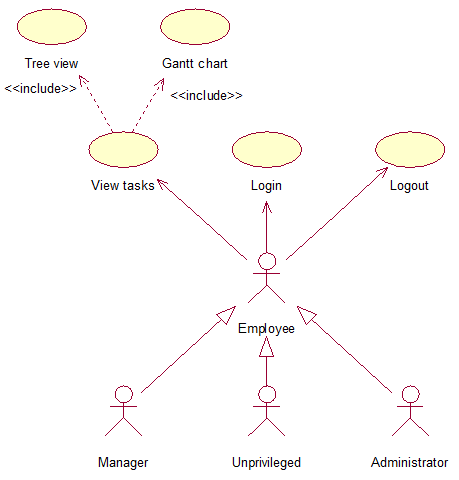
\includegraphics[scale=1]{diagrams/usecase1_2b.png} \end{center}
\caption{Use Case Diagram}
\label{fig:use-case-diagram}
\end{figure}
\begin{figure}[htbp]
\begin{center} 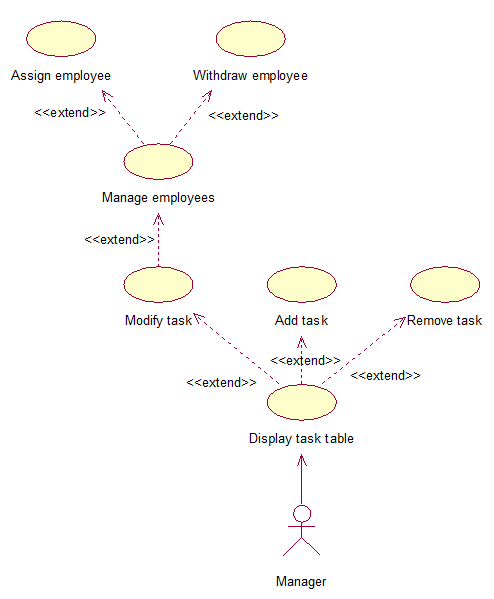
\includegraphics[scale=1]{diagrams/usecase1_2a.png} \end{center}
\caption{Use Case Diagram}
\label{fig:use-case-diagram}
\end{figure}
\begin{figure}[htbp]
\begin{center} 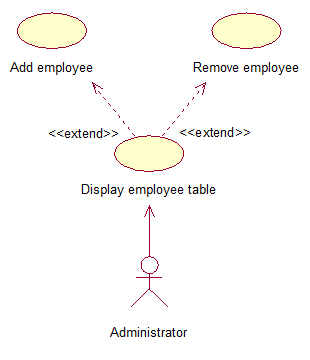
\includegraphics[scale=1]{diagrams/usecase1_2c.png} \end{center}
\caption{Use Case Diagram}
\label{fig:use-case-diagram}
\end{figure}

\subsubsection{Use Case 1} \label{uc:1}

\noindent
{\bf Name}\\
Login

\noindent
{\bf Summary}\\
The user requests access to the system. The user must be identified.

\noindent
{\bf Actors}\\
Any user.

\noindent
{\bf Precondition}\\
The system is active.

\noindent
{\bf Main Scenario}\\
\vspace*{-0.35in}
\begin{enumerate}
\item The system requests an identification (user name).
\vspace*{-0.1in}
\item The user selects their name from a list.
\vspace*{-0.1in}
\item The system grants the user access to the system.
\end{enumerate}
\vspace*{-0.1in}

\noindent
{\bf Exceptions}\\
\vspace*{-0.35in}
\begin{enumerate}
\item The person XML file is missing.
\end{enumerate}
\vspace*{-0.1in}

\noindent
{\bf Postcondition}\\
The user is granted access to the system.

\noindent
{\bf Priority}\\
Must.

\noindent
{\bf Traces to requirements}\\
F1, N1.

\subsubsection{Use Case 2} \label{uc:2}

\noindent
{\bf Name}\\
Logout

\noindent
{\bf Summary}\\
The user terminates their session.

\noindent
{\bf Actors}\\
Any user.

\noindent
{\bf Precondition}\\
The user is logged into the system.

\noindent
{\bf Main Scenario}\\
\vspace*{-0.35in}
\begin{enumerate}
\item The user clicks the ”logout” button available after login.
\vspace*{-0.1in}
\item The system terminates the session and requests a new identification.
\end{enumerate}
\vspace*{-0.1in}

\noindent
{\bf Postcondition}\\
The system remains active and awaits a new identification.

\noindent
{\bf Priority}\\
Must.

\noindent
{\bf Traces to requirements}\\
F1.

\subsubsection{Use Case 3} \label{uc:3}

\noindent
{\bf Name}\\
View tasks

\noindent
{\bf Summary}\\
The user requests a list of their tasks. They are presented with a menu from which they can choose different types of views for the data to be shown.

\noindent
{\bf Actors}\\
Any user.

\noindent
{\bf Precondition}\\
The user is in the ``view tasks" menu.

\noindent
{\bf Main Scenario}\\
\vspace*{-0.35in}
\begin{enumerate}
\item The user clicks the button that allows them to select a view.
\vspace*{-0.1in}
\item The system verifies the user's role.
\vspace*{-0.1in}
\item The system displays a list of different views, some views are specific to the user's role.
\end{enumerate}
\vspace*{-0.1in}

\noindent
{\bf Exceptions}\\
\vspace*{-0.35in}
\begin{enumerate}
\item The person XML file is missing.
\end{enumerate}
\vspace*{-0.1in}

\noindent
{\bf Postcondition}\\
The system displays a list of available views.

\noindent
{\bf Priority}\\
Must.

\noindent
{\bf Traces to requirements}\\
F6, F7.

\subsubsection{Use Case 4} \label{uc:4}

\noindent
{\bf Name}\\
Tree view

\noindent
{\bf Summary}\\
The user requests a dependency graph of their tasks.

\noindent
{\bf Actors}\\
Any user.

\noindent
{\bf Precondition}\\
The user has selected the tree view.

\noindent
{\bf Main Scenario}\\
\vspace*{-0.35in}
\begin{enumerate}
\item The user selects the tree view option.
\vspace*{-0.1in}
\item The system verifies the user's ID and role.
\vspace*{-0.1in}
\item The system constructs a dependency tree based of the user's tasks.
\vspace*{-0.1in}
\item The system renders and displays the graph.
\end{enumerate}
\vspace*{-0.1in}

\noindent
{\bf Exceptions}\\
\vspace*{-0.35in}
\begin{enumerate}
\item The person XML file is missing.
\vspace*{-0.1in}
\item The task XML file is missing.
\end{enumerate}
\vspace*{-0.1in}

\noindent
{\bf Postcondition}\\
The system displays a tree view.

\noindent
{\bf Priority}\\
Optional.

\noindent
{\bf Traces to requirements}\\
F6.

\subsubsection{Use Case 5} \label{uc:5}

\noindent
{\bf Name}\\
Gantt chart

\noindent
{\bf Summary}\\
The user requests a schedule of their tasks.

\noindent
{\bf Actors}\\
Any user.

\noindent
{\bf Precondition}\\
The user is in the ``view tasks" menu.

\noindent
{\bf Main Scenario}\\
\vspace*{-0.35in}
\begin{enumerate}
\item The user selects the gantt chart option.
\vspace*{-0.1in}
\item The system verifies the user's ID and role.
\vspace*{-0.1in}
\item The system constructs a schedule of the user's tasks.
\end{enumerate}
\vspace*{-0.1in}

\noindent
{\bf Exceptions}\\
\vspace*{-0.35in}
\begin{enumerate}
\item The person XML file is missing.
\vspace*{-0.1in}
\item The task XML file is missing.
\end{enumerate}
\vspace*{-0.1in}

\noindent
{\bf Postcondition}\\
The system displays a gantt chart.

\noindent
{\bf Priority}\\
Optional.

\noindent
{\bf Traces to requirements}\\
F7.

\subsubsection{Use Case 6} \label{uc:6}

\noindent
{\bf Name}\\
Display employee table

\noindent
{\bf Summary}\\
The user requests a table of all employees in order to manage them.

\noindent
{\bf Actors}\\
Administrators.

\noindent
{\bf Precondition}\\
The user must be logged in.

\noindent
{\bf Main Scenario}\\
\vspace*{-0.35in}
\begin{enumerate}
\item The user selects the employee table button.
\vspace*{-0.1in}
\item The system constructs a table of all employees.
\vspace*{-0.1in}
\item The system renders and displays the employee table.
\end{enumerate}
\vspace*{-0.1in}

\noindent
{\bf Exceptions}\\
\vspace*{-0.35in}
\begin{enumerate}
\item The person XML file is missing.
\end{enumerate}
\vspace*{-0.1in}

\noindent
{\bf Postcondition}\\
The system displays a view of the current employees and options related to employee management.

\noindent
{\bf Priority}\\
Must.

\noindent
{\bf Traces to requirements}\\
F10, F11, F12.

\subsubsection{Use Case 7} \label{uc:7}

\noindent
{\bf Name}\\
Add employee

\noindent
{\bf Summary}\\
The user wants to add an employee into the system.

\noindent
{\bf Actors}\\
Administrators.

\noindent
{\bf Precondition}\\
The user is in the employee table view.

\noindent
{\bf Main Scenario}\\
\vspace*{-0.35in}
\begin{enumerate}
\item The user selects the option to add a new employee.
\vspace*{-0.1in}
\item The system requests information about the new employee.
\vspace*{-0.1in}
\item The user submits the information.
\vspace*{-0.1in}
\item The system adds the employee into the system.
\end{enumerate}
\vspace*{-0.1in}

\noindent
{\bf Exceptions}\\
\vspace*{-0.35in}
\begin{enumerate}
\item The person XML file is missing.
\end{enumerate}
\vspace*{-0.1in}

\noindent
{\bf Postcondition}\\
A new employee is added into the system.

\noindent
{\bf Priority}\\
Must.

\noindent
{\bf Traces to requirements}\\
F11.

\subsubsection{Use Case 8} \label{uc:8}

\noindent
{\bf Name}\\
Remove employee

\noindent
{\bf Summary}\\
The user wants to remove an employee.

\noindent
{\bf Actors}\\
Administrator.

\noindent
{\bf Precondition}\\
The user is in the employee table view.

\noindent
{\bf Main Scenario}\\
\vspace*{-0.35in}
\begin{enumerate}
\item The user selects the option to remove a specific employee.
\vspace*{-0.1in}
\item The system confirms his request.
\vspace*{-0.1in}
\item The system removes the employee.
\end{enumerate}
\vspace*{-0.1in}

\noindent
{\bf Exceptions}\\
\vspace*{-0.35in}
\begin{enumerate}
\item The person XML file is missing.
\end{enumerate}
\vspace*{-0.1in}

\noindent
{\bf Postcondition}\\
An  employee is removed from the system.

\noindent
{\bf Priority}\\
Must.

\noindent
{\bf Traces to requirements}\\
F12.

\subsubsection{Use Case 9} \label{uc:9}

\noindent
{\bf Name}\\
Display task table

\noindent
{\bf Summary}\\
The user wants to see a view of tasks in order to manage them.

\noindent
{\bf Actors}\\
Managers.

\noindent
{\bf Precondition}\\
The user must be logged in.

\noindent
{\bf Main Scenario}\\
\vspace*{-0.35in}
\begin{enumerate}
\item The user requests to see the task table.
\vspace*{-0.1in}
\item The system shows the user a table with tasks and offers task management options.
\end{enumerate}
\vspace*{-0.1in}

\noindent
{\bf Exceptions}\\
\vspace*{-0.35in}
\begin{enumerate}
\item The person XML file is missing.
\vspace*{-0.1in}
\item The task XML file is missing.
\end{enumerate}
\vspace*{-0.1in}

\noindent
{\bf Postcondition}\\
A view is shown to the user that shows current tasks and options related to task management.

\noindent
{\bf Priority}\\
Must.

\noindent
{\bf Traces to requirements}\\
F2, F3, F4, F5, F8, F9, F13.

\subsubsection{Use Case 10} \label{uc:10}

\noindent
{\bf Name}\\
Add task

\noindent
{\bf Summary}\\
The user wants to add a task to the pool of tasks.

\noindent
{\bf Actors}\\
Managers.

\noindent
{\bf Precondition}\\
The user is in the task table view.

\noindent
{\bf Main Scenario}\\
\vspace*{-0.35in}
\begin{enumerate}
\item The user requests to add a task.
\vspace*{-0.1in}
\item The system requests information on the task to be added.
\vspace*{-0.1in}
\item The user submits the information.
\vspace*{-0.1in}
\item The system creates the task.
\end{enumerate}
\vspace*{-0.1in}

\noindent
{\bf Exceptions}\\
\vspace*{-0.35in}
\begin{enumerate}
\item The person XML file is missing.
\vspace*{-0.1in}
\item The task XML file is missing.
\end{enumerate}
\vspace*{-0.1in}

\noindent
{\bf Postcondition}\\
A new task is added into the system.

\noindent
{\bf Priority}\\
Must.

\noindent
{\bf Traces to requirements}\\
F3.

\subsubsection{Use Case 11} \label{uc:11}

\noindent
{\bf Name}\\
Remove task

\noindent
{\bf Summary}\\
The user wants to remove a task from the pool of tasks.

\noindent
{\bf Actors}\\
Managers.

\noindent
{\bf Precondition}\\
The user is in the task table view.

\noindent
{\bf Main Scenario}\\
\vspace*{-0.35in}
\begin{enumerate}
\item The user requests to remove a specific task.
\vspace*{-0.1in}
\item The system confirms his request.
\vspace*{-0.1in}
\item The system removes the task.
\end{enumerate}
\vspace*{-0.1in}

\noindent
{\bf Exceptions}\\
\vspace*{-0.35in}
\begin{enumerate}
\item The task XML file is missing.
\end{enumerate}
\vspace*{-0.1in}

\noindent
{\bf Postcondition}\\
A task is removed from the system.

\noindent
{\bf Priority}\\
Must.

\noindent
{\bf Traces to requirements}\\
F4.

\subsubsection{Use Case 12} \label{uc:12}

\noindent
{\bf Name}\\
Modify task

\noindent
{\bf Summary}\\
The user wants to modify a task in the pool of tasks and is given the option to manage employees related to that task.

\noindent
{\bf Actors}\\
Managers.

\noindent
{\bf Precondition}\\
The user is in the task table view.

\noindent
{\bf Main Scenario}\\
\vspace*{-0.35in}
\begin{enumerate}
\item The user requests to modify a specific task.
\vspace*{-0.1in}
\item The system displays a menu that shows properties of task and allows the user to modify them.
\vspace*{-0.1in}
\item The system confirms his request.
\vspace*{-0.1in}
\item The system modifies the task.
\end{enumerate}
\vspace*{-0.1in}

\noindent
{\bf Exceptions}\\
\vspace*{-0.35in}
\begin{enumerate}
\item The person XML file is missing.
\vspace*{-0.1in}
\item The task XML file is missing.
\end{enumerate}
\vspace*{-0.1in}

\noindent
{\bf Postcondition}\\
A previously created task is modified.

\noindent
{\bf Priority}\\
Must.

\noindent
{\bf Traces to requirements}\\
F5, F8, F9, F13.

\subsubsection{Use Case 13} \label{uc:13}

\noindent
{\bf Name}\\
Manage employees

\noindent
{\bf Summary}\\
The user wants to manage employees on a previously created task.

\noindent
{\bf Actors}\\
Managers.

\noindent
{\bf Precondition}\\
The user must be modifying a task.

\noindent
{\bf Main Scenario}\\
\vspace*{-0.35in}
\begin{enumerate}
\item The user requests to manage employees.
\vspace*{-0.1in}
\item An option menu appears to the user to give a choice of how to manage his employees.
\end{enumerate}
\vspace*{-0.1in}

\noindent
{\bf Exceptions}\\
\vspace*{-0.35in}
\begin{enumerate}
\item The person XML file is missing.
\vspace*{-0.1in}
\item The task XML file is missing.
\end{enumerate}
\vspace*{-0.1in}

\noindent
{\bf Postcondition}\\
A menu appears to show the user how he can manage employees.

\noindent
{\bf Priority}\\
Must.

\noindent
{\bf Traces to requirements}\\
F8, F9, F13.

\subsubsection{Use Case 14} \label{uc:14}

\noindent
{\bf Name}\\
Assign employee

\noindent
{\bf Summary}\\
The user wants to assign an employee to a task.

\noindent
{\bf Actors}\\
Managers.

\noindent
{\bf Precondition}\\
The user must be in the manage employees menu.

\noindent
{\bf Main Scenario}\\
\vspace*{-0.35in}
\begin{enumerate}
\item The user chooses to assign an employee to the task.
\vspace*{-0.1in}
\item The system shows a list of employees that can be assigned.
\vspace*{-0.1in}
\item The user selects an employee.
\vspace*{-0.1in}
\item The system updates the task.
\end{enumerate}
\vspace*{-0.1in}

\noindent
{\bf Exceptions}\\
\vspace*{-0.35in}
\begin{enumerate}
\item The person XML file is missing.
\vspace*{-0.1in}
\item The task XML file is missing.
\vspace*{-0.1in}
\item No employees are registered into the system.
\end{enumerate}
\vspace*{-0.1in}

\noindent
{\bf Postcondition}\\
An employee is assigned to a task.

\noindent
{\bf Priority}\\
Must.

\noindent
{\bf Traces to requirements}\\
F9.

\subsubsection{Use Case 15} \label{uc:15}

\noindent
{\bf Name}\\
Withdraw employee

\noindent
{\bf Summary}\\
The user wants to withdraw an employee from a task.

\noindent
{\bf Actors}\\
Managers.

\noindent
{\bf Precondition}\\
The user must be in the manage employees menu.

\noindent
{\bf Main Scenario}\\
\vspace*{-0.35in}
\begin{enumerate}
\item The user chooses to remove an employee from the task.
\vspace*{-0.1in}
\item The system shows a list of people that are assigned to the task.
\vspace*{-0.1in}
\item The user selects an employee.
\vspace*{-0.1in}
\item The system confirms the choice of the user.
\vspace*{-0.1in}
\item The system removes the employee from the task.
\end{enumerate}
\vspace*{-0.1in}

\noindent
{\bf Exceptions}\\
\vspace*{-0.35in}
\begin{enumerate}
\item The person XML file is missing.
\vspace*{-0.1in}
\item The task XML file is missing.
\vspace*{-0.1in}
\item No employees are assigned on the task.
\end{enumerate}
\vspace*{-0.1in}

\noindent
{\bf Postcondition}\\
An employee is withdrawn from a task.

\noindent
{\bf Priority}\\
Must.

\noindent
{\bf Traces to requirements}\\
F13.

\section{Functional requirements}

\subsubsection{F1} \label{uc:1}

\noindent
{\bf Requirement}\\
Only one person should be logged in at a time.

\noindent
{\bf Rationale}\\
Different actors have access to different functionalities in the system.

\noindent
{\bf Priority}\\
Must.

\noindent
{\bf Traces to use cases}\\
Login, logout.

\subsubsection{F2} \label{uc:2}

\noindent
{\bf Requirement}\\
A view of tasks in the company is to be shown to the user in order for him to manage them.

\noindent
{\bf Rationale}\\
A manager can manage tasks and assign employees to work on them.

\noindent
{\bf Priority}\\
Must.

\noindent
{\bf Traces to use cases}\\
Display task table.

\subsubsection{F3} \label{uc:3}

\noindent
{\bf Requirement}\\
The user is to be able to enter a new task.

\noindent
{\bf Rationale}\\
A manager must be able to create new tasks in order to help him manage his employees' time.

\noindent
{\bf Priority}\\
Must.

\noindent
{\bf Traces to use cases}\\
Display task table, add task

\subsubsection{F4} \label{uc:4}

\noindent
{\bf Requirement}\\
The user is to be able to remove a previously created task.

\noindent
{\bf Rationale}\\
A manager must be able to remove tasks in order to help him manage his employees' time.

\noindent
{\bf Priority}\\
Must.

\noindent
{\bf Traces to use cases}\\
Display task table, remove task.

\subsubsection{F5} \label{uc:5}

\noindent
{\bf Requirement}\\
The user is to be able to modify a previously created task.

\noindent
{\bf Rationale}\\
A manager must be able to modify tasks in order to help him manage his employees' time.

\noindent
{\bf Priority}\\
Must.

\noindent
{\bf Traces to use cases}\\
Display task table, modify task.

\subsubsection{F6} \label{uc:6}

\noindent
{\bf Requirement}\\
The user is to be able to view a dependency graph of tasks.

\noindent
{\bf Rationale}\\
The user must be able to view the dependency relations between tasks in order for him to manage his own time.

\noindent
{\bf Priority}\\
Optional.

\noindent
{\bf Traces to use cases}\\
View tasks, Tree view.

\subsubsection{F7} \label{uc:7}

\noindent
{\bf Requirement}\\
The user is to be able to view a Gantt chart of tasks.

\noindent
{\bf Rationale}\\
The user must be able to view the a schedule of their tasks in order for him to manage his own time.

\noindent
{\bf Priority}\\
Optional.

\noindent
{\bf Traces to use cases}\\
View tasks, Gantt chart.

\subsubsection{F8} \label{uc:8}

\noindent
{\bf Requirement}\\
The user must be able to manage employees on a task.

\noindent
{\bf Rationale}\\
A manager must be able to modify the list of employees that are working on a task.

\noindent
{\bf Priority}\\
Must.

\noindent
{\bf Traces to use cases}\\
Display task table, modify task, Manage employees

\subsubsection{F9} \label{uc:9}

\noindent
{\bf Requirement}\\
The user must be able to assign employees to a task.

\noindent
{\bf Rationale}\\
A manager must be able to assign an employee to a task in order for the employee to receive information about the task.

\noindent
{\bf Priority}\\
Must.

\noindent
{\bf Traces to use cases}\\
Display task table, modify task, manage employees, assign employee.

\subsubsection{F10} \label{uc:10}

\noindent
{\bf Requirement}\\
The user must be able to view a list of employees in the company in order for him to manage them.

\noindent
{\bf Rationale}\\
An administrator has to manage the workforce of the company since these might change during the course of a project.

\noindent
{\bf Priority}\\
Must.

\noindent
{\bf Traces to use cases}\\
Display employee table, add employee, remove employee.

\subsubsection{F11} \label{uc:11}

\noindent
{\bf Requirement}\\
The user is to be able to add a new employee.

\noindent
{\bf Rationale}\\
An administrator must be able to add new employees into the system when hired to work on the project.

\noindent
{\bf Priority}\\
Must.

\noindent
{\bf Traces to use cases}\\
Add employee.

\subsubsection{F12} \label{uc:12}

\noindent
{\bf Requirement}\\
The user is to be able to remove an employee.

\noindent
{\bf Rationale}\\
An administrator must be able to remove employees from the system when they cease to work on the project.

\noindent
{\bf Priority}\\
Must.

\noindent
{\bf Traces to use cases}\\
Remove employee.

\subsubsection{F13} \label{uc:13}

\noindent
{\bf Requirement}\\
The user must be able to withdraw employees from a task.

\noindent
{\bf Rationale}\\
A manager must be able to withdraw an employee from a task to stop the system from showing information about the task to that employee.

\noindent
{\bf Priority}\\
Must.

\noindent
{\bf Traces to use cases}\\
Display task table, modify task, manage employees, Withdraw employee.

\section{Non-Functional requirements}

\subsubsection{N1} \label{uc:N1}

\noindent
{\bf Requirement}\\
The system must know who the user is in order to offer the appropriate options.

\noindent
{\bf Rationale}\\
Different actors should have different options available to them.

\noindent
{\bf Priority}\\
Must.

\noindent
{\bf Traces to use cases}\\
Login.

\subsubsection{O1} \label{uc:O1}

\noindent
{\bf Requirement}\\
It shall be possible to run the system on any computer system that runs the JVM.

\noindent
{\bf Rationale}\\
The system should be accessible to the largest customer base, regardless of their OS.

\noindent
{\bf Priority}\\
Optional.

\noindent
{\bf Traces to use cases}\\
All use cases.

\section{References}

\pagebreak

\appendix

\section{Description of File Format: tasks.xml}

\texttt{<tasks>} : Root node used to specify the beginning of the listing of tasks \\

\texttt{<task>} : Node used to specify a new task \\

\texttt{<identifier>} : A unique, alphanumberic identifier for each task \\

\texttt{<title>} : Node to store a short title for the task \\

\texttt{<description>} : Node to store a full description for the task \\

\texttt{<startdate>} : Node to store the appropriate start date for the task \\

\texttt{<duration>} : The duration, in hours of the task. \\

\texttt{<deliverable>} : The expected physical deliverable upon task completion \\

\texttt{<deadline>} : The date by which the task must be completed \\

\texttt{<peopleassigned>} : A listing of the individuals assigned to the task.
The duration will be split evenly among assignees. \\

\texttt{<id>} : The corresponding identifier for each person assigned \\

\texttt{<completion>} : The percentage of completion for the task \\

\pagebreak

\section{Description of File Format: people.xml}

\texttt{<people>} : Root node used to specify the beginning of the listing of people \\

\texttt{<person>} : Node used to specify a new person \\

\texttt{<identifier>} : A unique, alphanumberic identifier for each person \\

\texttt{<fname>} : Node used to store the first name of the person \\

\texttt{<lname>} : Node used to store the last name of the person \\

\texttt{<jobtitle>} : Node used to track the job title of the person.
Used to differentiate between roles \\

\texttt{<jobdescription>} : Node used for the person's job description. \\

\texttt{<clearance>} : Node used to specify the clearance a person within the organization.
Restricts permission based on value. 0 - Employee, 1 - Manager, 2 - Administrator \\

\section{Description of File Format: people.txt}

The list of people with a summary of their names, the total amount of time
spent on all projects, and the specific projects to which they are assigned.

\begin{lstlisting}
Name                | Total Hours        | Project List              
---------------------------------------------------------
LName, FName        | X.X                | A, B, C
\end{lstlisting}

\end{document}
